\subsubsection{Everything step-by-step}

A top-down list of everything in section \ref{sec:color_basic}, \ref{sec:color_properties_tool} and \ref{sec:color_dir_highlight}. Concentrating on what to actually do, without much explanation.

\begin{enumerate}[a)]
    
    \item Get ColorTool from Microsoft in order to set a theme.
    \begin{enumerate}[1.]
        \item Go to \url{https://github.com/microsoft/terminal/tree/master/src/tools/ColorTool}
    
        \item Click the link under the title \textbf{Installing} in \texttt{README.md} in order to see the latest release.\\E.g. \url{https://github.com/microsoft/terminal/releases/tag/1904.29002}
        
        \item Download the ColorTool zip file.
    \end{enumerate}
    
    \item Activate a theme with ColorTool.
    \begin{enumerate}[1.]
        \item Open \texttt{Command Prompt} in Windows.
        
        \item In \texttt{CMD} look at the PATH variable with \code{PATH} or \code{echo \%PATH\%}
        
        \item Copy one of the locations shown to store the ColorTool and color scheme.\\E.g. \code{C:\Users\Robin.Hellmers\AppData\Local\Microsoft\WindowsApps}
        
        \item Unzip the files in that location.
        
        \item Go to the very same directory in \texttt{CMD} with\\E.g. \code{cd C:\Users\Robin.Hellmers\AppData\Local\Microsoft\WindowsApps}
        
        \item In the \texttt{CMD}, run \code{ColorTool -b solarized\_dark.itermcolors}.
        
        \item Restart the \texttt{Ubuntu} terminal.
    \end{enumerate}
    
    \item Fix directory highlight inconsistency (Different permissions for \texttt{Windows} and \texttt{Ubuntu}).
    \begin{enumerate}[1.]
        \item In the \texttt{Ubuntu} terminal, run \code{dircolors -p > ~/.dircolors}
        
        \item Find \code{DIR}, \code{STICKY\_OTHER\_VARIABLE}, \code{STICKY} and write their corresponding values in the comments in case one want to revert the upcoming changes.
        
        \item Find \code{OTHER\_WRITABLE} and copy the variable value e.g. \code{34;42}.
        
        \item Replace the values of \code{DIR}, \code{STICKY\_OTHER\_VARIABLE}, \code{STICKY} with the copied value.
        
        \item Restart the \texttt{Ubuntu} terminal.
    \end{enumerate}
    
    \item Set specific colors with the properties tool
    \begin{itemize}
        \item BE CAREFUL, weird tool
        
        \item In order to revert back
        \begin{enumerate}[a)]
            \item Open the \texttt{Registry editor (regedit)} and\\remove \code{HKEY\_CURRENT\_USER\Console\something\_with\_ubuntu\_in\_the\_name}.
            
            \item Open up \textbf{Properties} and the \textbf{Colors} tab. Click \texttt{OK} to recreate the registry which you removed.
        \end{enumerate}
    \end{itemize}
    \begin{enumerate}[1.]
        \item Open the \texttt{Ubuntu} terminal.
        
        \item Right-click on the top bar which says e.g. \textbf{Ubuntu 18.04 LTS} to the right of the icon logo. Press \textbf{Properties} and go to the \textbf{Color} tab.
        \begin{figure}[H]
            \centering
            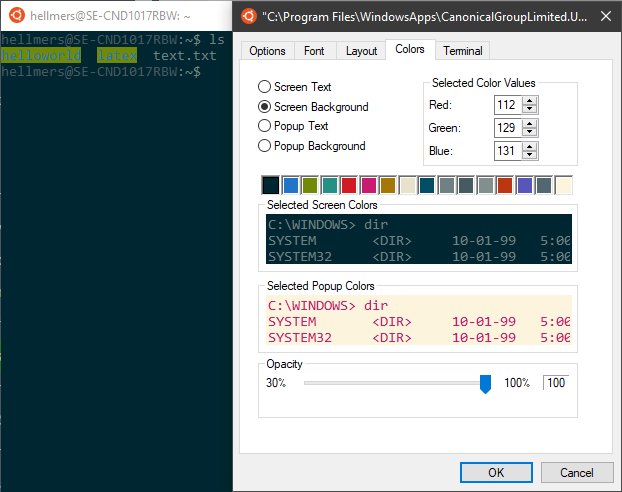
\includegraphics[width=0.75\textwidth]{tex/WSL/Ubuntu_terminal_colors/Figures/1.PNG}
        \end{figure}
        
        \item Click between \textbf{Screen Background} and \textbf{Screen Text} in order to see which colors are highlighted and chosen as standard for each. Remember which is highlighted for which (main colors).
        \begin{itemize}
            \item In order to see the RGB values, you must click on the highlighted color. But beware that the color which you select must be the highlighted one for that specific category e.g. \textbf{Screen Background} or else you will change it.
        \end{itemize}
        \begin{figure}[H]
            \centering
            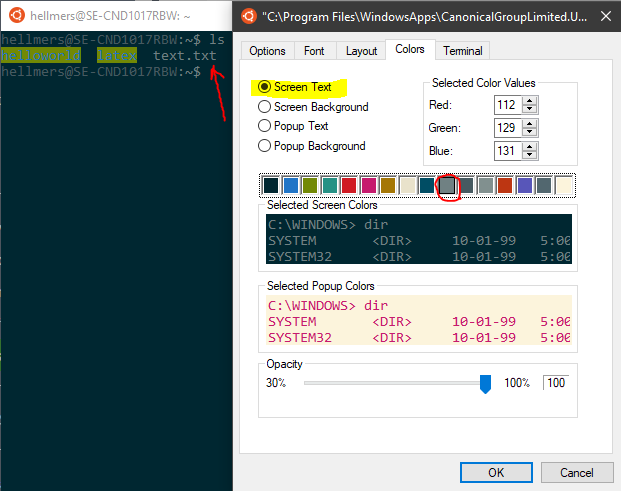
\includegraphics[width=0.75\textwidth]{tex/WSL/Ubuntu_terminal_colors/Figures/2.PNG}
        \end{figure}
        \begin{figure}[H]
            \centering
            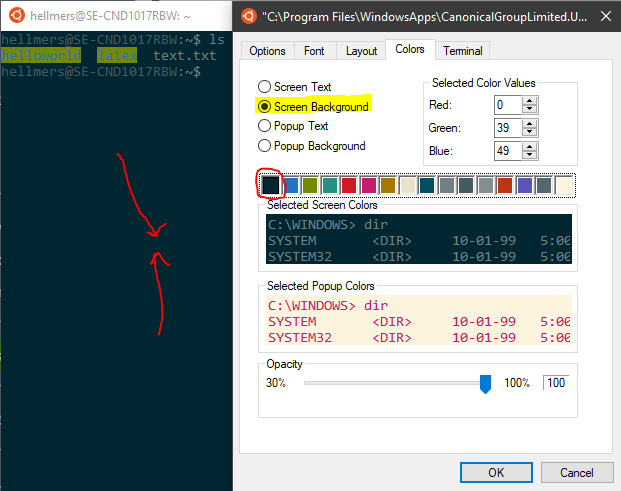
\includegraphics[width=0.75\textwidth]{tex/WSL/Ubuntu_terminal_colors/Figures/3.PNG}
        \end{figure}
        
        \item Choose \textbf{Screen Background} and select the 3rd color (green).
        \begin{figure}[H]
            \centering
            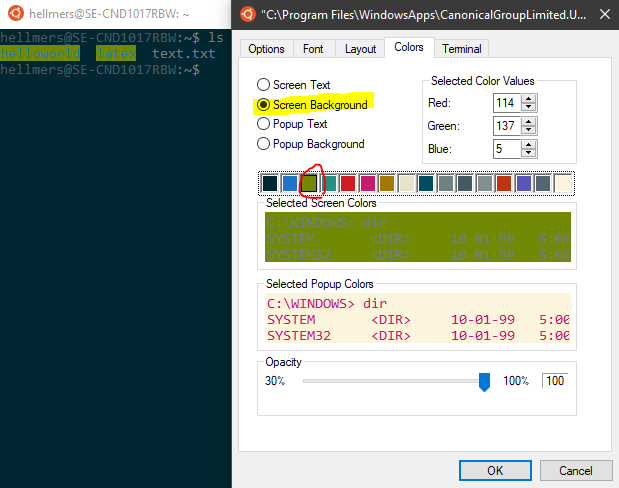
\includegraphics[width=0.75\textwidth]{tex/WSL/Ubuntu_terminal_colors/Figures/4.PNG}
        \end{figure}
        
        \item Replace the RGB colors to the same as the figure below.
        \begin{figure}[H]
            \centering
            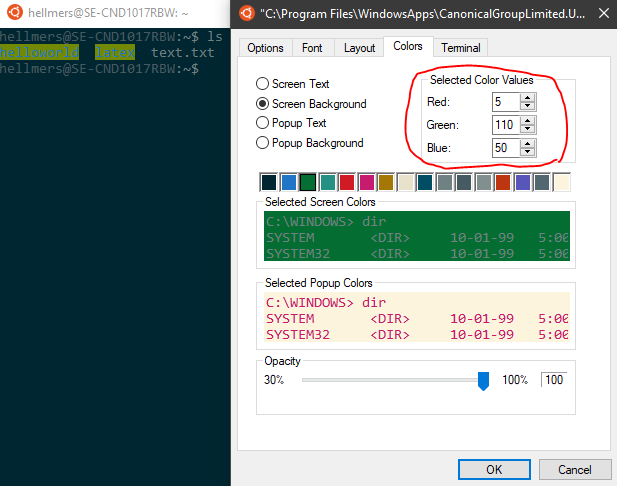
\includegraphics[width=0.75\textwidth]{tex/WSL/Ubuntu_terminal_colors/Figures/5.PNG}
        \end{figure}
        
        \item Choose \textbf{Screen Text} and select the 2nd color (blue).
        \begin{figure}[H]
            \centering
            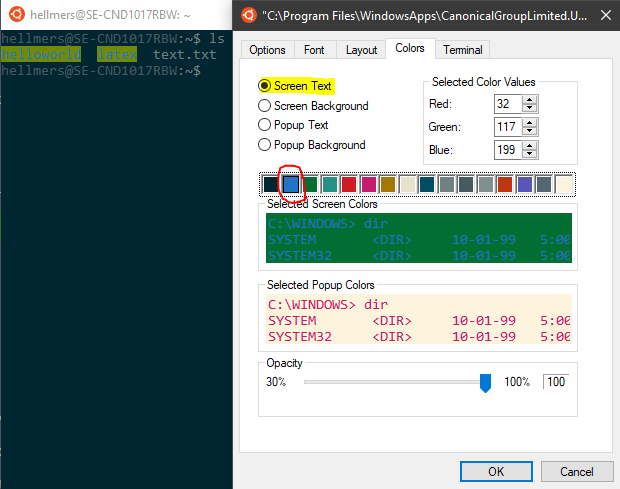
\includegraphics[width=0.75\textwidth]{tex/WSL/Ubuntu_terminal_colors/Figures/6.PNG}
        \end{figure}
        
        \item Replace the RGB colors to the same as the figure below.
        \begin{figure}[H]
            \centering
            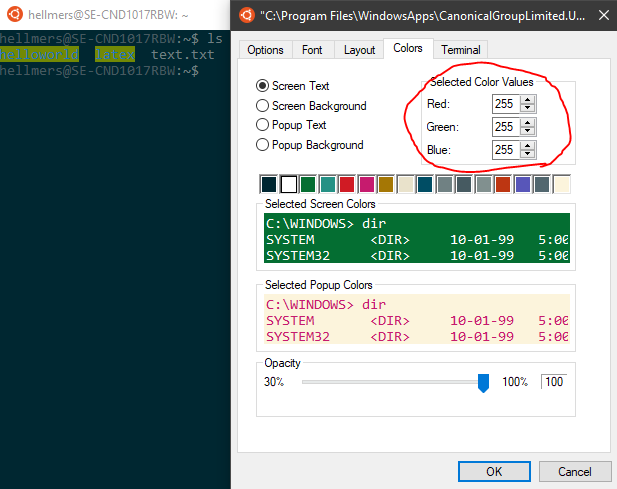
\includegraphics[width=0.75\textwidth]{tex/WSL/Ubuntu_terminal_colors/Figures/7.PNG}
        \end{figure}
        
        \item Choose \textbf{Screen Background} and select the main color for \textbf{Screen Background}.
        \begin{figure}[H]
            \centering
            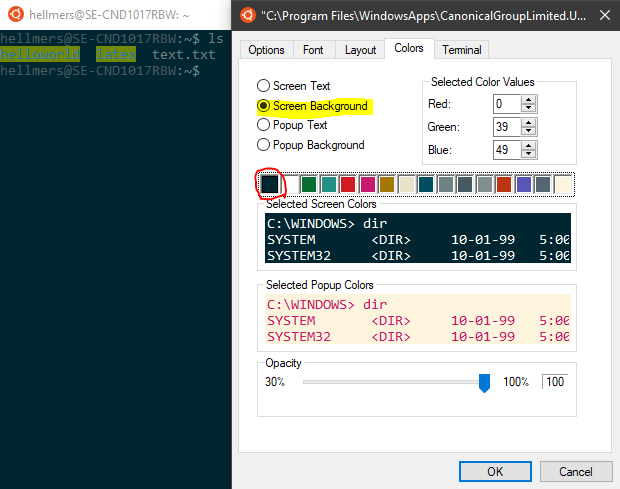
\includegraphics[width=0.75\textwidth]{tex/WSL/Ubuntu_terminal_colors/Figures/8.PNG}
        \end{figure}
        
        \item Choose \textbf{Screen Text} and select the main color for \textbf{Screen Text}.
        \begin{figure}[H]
            \centering
            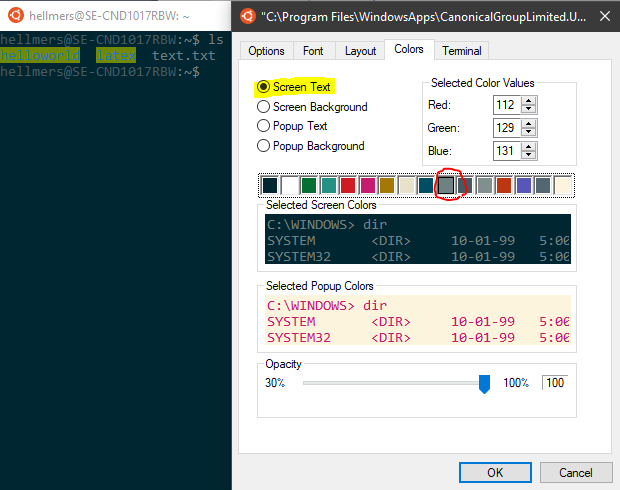
\includegraphics[width=0.75\textwidth]{tex/WSL/Ubuntu_terminal_colors/Figures/9.PNG}
        \end{figure}
        
        \item Press \texttt{OK} to save the changes.
        \begin{figure}[H]
            \centering
            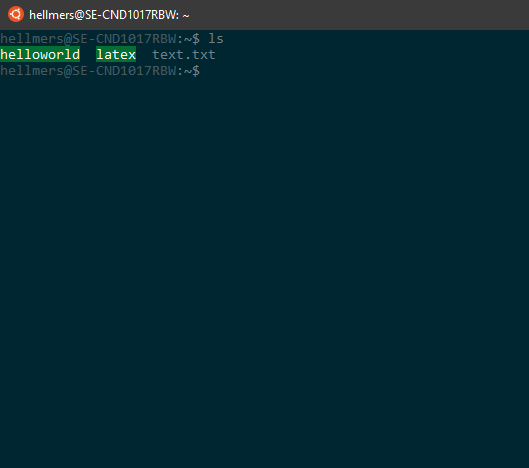
\includegraphics[width=0.75\textwidth]{tex/WSL/Ubuntu_terminal_colors/Figures/10.PNG}
        \end{figure}
        
        \item Open up \textbf{Properties} and the \textbf{Colors} tab again.
        
        \item Choose \textbf{Screen Text} and select the 11th color (grey).
        \begin{figure}[H]
            \centering
            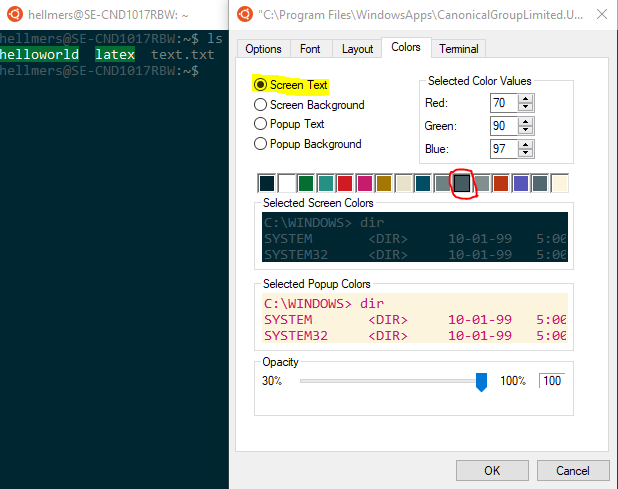
\includegraphics[width=0.75\textwidth]{tex/WSL/Ubuntu_terminal_colors/Figures/11.PNG}
        \end{figure}
        
        \item Replace the RGB colors to the same as the figure below.
        \begin{figure}[H]
            \centering
            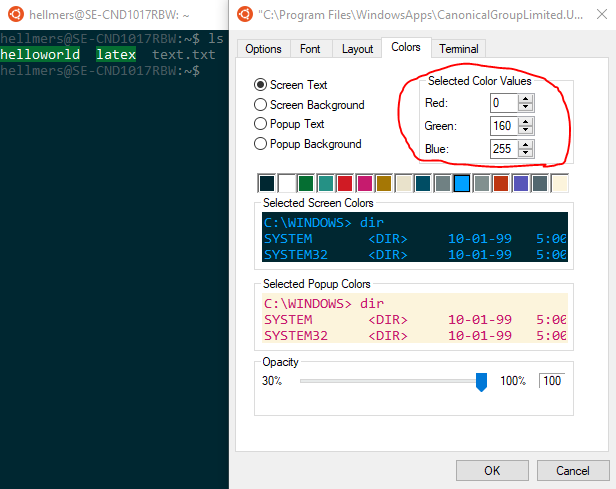
\includegraphics[width=0.75\textwidth]{tex/WSL/Ubuntu_terminal_colors/Figures/12.PNG}
        \end{figure}
        
        \item Select the main color for \textbf{Screen Text}.
        \begin{figure}[H]
            \centering
            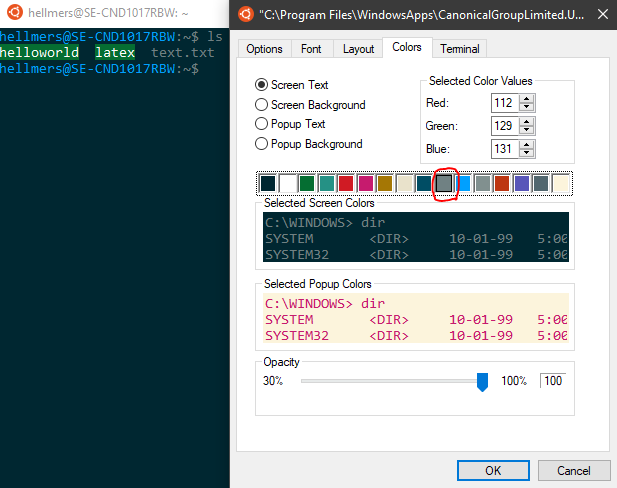
\includegraphics[width=0.75\textwidth]{tex/WSL/Ubuntu_terminal_colors/Figures/13.PNG}
        \end{figure}
        
        \item Replace the RGB colors to the same as the figure below.
        \begin{figure}[H]
            \centering
            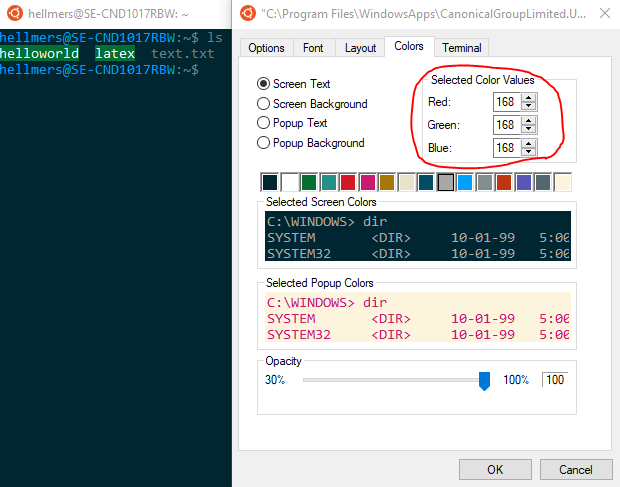
\includegraphics[width=0.75\textwidth]{tex/WSL/Ubuntu_terminal_colors/Figures/14.PNG}
        \end{figure}
        
        \item Click \texttt{OK} to save the changes.
        \begin{figure}[H]
            \centering
            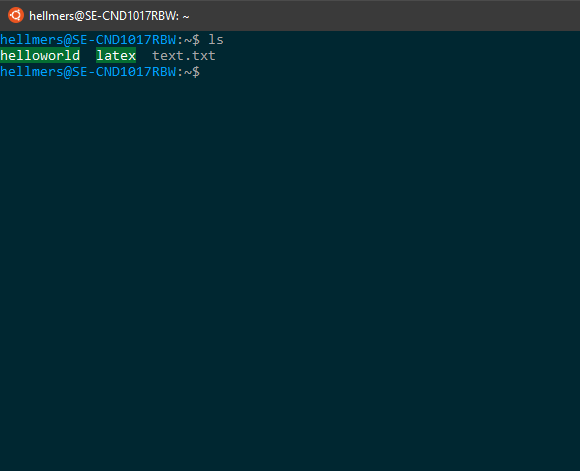
\includegraphics[width=0.75\textwidth]{tex/WSL/Ubuntu_terminal_colors/Figures/15.PNG}
        \end{figure}
    \end{enumerate}
    
    \item Change \code{vimdiff} colors
    \begin{enumerate}[1.]
        \item Create the directory \code{~/.vim/colors/}.
        
        \item Create the file \code{~/.vim/color/mycolorscheme.vim}
        
        \item Paste this into the file (see \href{https://github.com/robinhellmers/computer_setup/blob/master/vimdiff_colors/vim/colors/mycolorscheme.vim}{Github}):
\begin{minted}[tabsize=3,obeytabs,bgcolor=codegray]{bash}
highlight DiffAdd    cterm=bold ctermfg=15 ctermbg=22 gui=none guifg=bg guibg=Red
highlight DiffDelete cterm=bold ctermfg=15 ctermbg=88 gui=none guifg=bg guibg=Red
highlight DiffChange cterm=bold ctermfg=15 ctermbg=17 gui=none guifg=bg guibg=Red
highlight DiffText   cterm=bold ctermfg=15 ctermbg=130 gui=none guifg=bg guibg=Red
\end{minted}
        
        \item Create the file \code{~/.vimrc}
        
        \item Paste this into the file (see \href{https://github.com/robinhellmers/computer_setup/blob/master/vimdiff_colors/vimrc}{Github}):
\begin{minted}{bash}
if &diff
    colorscheme mycolorscheme
endif
\end{minted}
        
        \item Now the custom color scheme should be applied every time you open \code{vimdiff}.
    \end{enumerate}
    
\end{enumerate}


